\section{adaptive\_clustering\_X} \label{sec-adaptive-clust}

\subsection{General}
The adaptive clustering tools are at the heart of the MNHN-Tree-Tools suite.
The adaptive clustering tools perform a progressive scan using
different densities in exploiting the DBSCAN \cite{dbscan} algorithm in order to
build trees, and gain further insight into a dataset of
sequences. Just as the DBSCAN clustering tools (c.f. section
\ref{sec-dbscan-cluster}), the adaptive
clustering algorithm exists in different variants, corresponding to
sequence distance measure and underlying machine hardware. The tools
are: \emph{adaptive\_clustering\_PCA}, \emph{adaptive\_clustering\_kmer\_L1},
\emph{adaptive\_clustering\_kmer\_L2}, \emph{adaptive\_clustering\_SW\_GPU},
\emph{adaptive\_clustering\_SW\_MPI\_GPU} 

\subsection{Usage}

One can call the utilities with the following commands: 

\lstset{language=bash,
  caption={Calling the \emph{adaptive\_clustering\_X} tools},
  label=lst-adaptive-call}
\begin{lstlisting}
adaptive_clustering_PCA [fasta] [initial-epsilon] [delta-epsilon] \
   [minPoints] [split-sets] [n-threads] [dimensions] [pca-file] > [outfile]

adaptive_clustering_kmer_L1 [kmers] [initial-epsilon] [delta-epsilon] \
   [minPoints] [split-sets] [n-threads] > [outfile]

adaptive_clustering_kmer_L2 [kmers] [initial-epsilon] [delta-epsilon] \
   [minPoints] [split-sets] [n-threads] > [outfile]

adaptive_clustering_SW [fasta] [initial-epsilon] [delta-epsilon] \
  [minPoints] [split-sets] [n-threads] > [outfile]

adaptive_clustering_SW_GPU [fasta] [initial-epsilon] [delta-epsilon] \
   [minPoints] [split-sets] [n-threads] > [outfile]

adaptive_clustering_SW_MPI_GPU [fasta] [initial-epsilon] [delta-epsilon] \
   [minPoints] [split-sets] [n-threads] > [outfile]
\end{lstlisting}
which have the following arguments:
\begin{enumerate}
  \item \emph{fasta} The FASTA file containing the dataset to be
    adaptive clustered and to have a tree built from.
  \item \emph{kmers} A k-mer representation of a dataset to be
    adaptive clustered and to have a tree built from. Such a set can
    be obtained by the \emph{fasta2kmer} tool highlighted in section
    \ref{sec-fasta2kmer}
  \item \emph{initial-epsilon} The initial epsilon to start an adaptive
    clustering run from.
  \item \emph{delta-epsilon} The increase in epsilon between
    successive calls of the DBSCAN algorithm.
  \item \emph{minPoints} The number of sequences need to be found
    within an epsilon neighborhood to form or expand a cluster.
  \item \emph{split-sets} A split is a binary file to hold entire clustering
    results. As the algorithm creates multiple split sets ( one for
    each stage of the tree ) a path with a named prefix has to be
    given. The splitsets are named by the argument given with a
    running number at the end starting at 0 for the outermost leaves
    of the tree counting upwards until only a single cluster can be
    formed, the one with the lowest density.
  \item \emph{n-threads} The number of threads this run can be allowed
    to use. MPI\_GPU runs will fail if this value is not set to 1.
  \item \emph{outfile} The outfile of the adaptive clustering run
    which is valuable not only for informative purposes but also for
    further tools of this software suite.
\end{enumerate}

\subsection{Algorithm}

The algorithm resides on the DBSCAN algorithm already outlined in
section \ref{sec-dbscan-cluster}. The algorithm starts at a given
sequence density defined by the parameters \emph{initial-epsilon} and
\emph{minPoints}, as highlighted by equation \ref{eqn-density}. By
successive increasing $\epsilon$ by \emph{delta-epsilon} and hence
successive DBSCAN runs several clusterings with ever decreased
densities are generated. Clusterings with contain a higher or the same
number of clusters as the previous DBSCAN runs are discarded, only
clustering results with less clusters in lesser density run are kept,
until a system with a single cluster is reached. We further remark
that a result can be obtained at any specified density à posteriory if
the researcher requests to do so with the \emph{cluster\_dbscan\_X}
tools highlighted in section \ref{sec-dbscan-cluster}. We shall also
outline that this forced monotony in an every decreasing number of
clusters also makes the importance of a wisely chosen starting point:
\emph{initial-epsilon} and \emph{minpoints} necessary. The starting
point shall be chooses at a density where the highest number of
clusters is suspected.
From these multiple clustering results at different densities we can
infer a hierarchy by comparing clusters of different layers and
verifying weather they assumed smaller clusters at higher densities
are a part of larger clusters in results from cluster runs at lesser
densities. Connections between clusters are created and print to the
output file if a cluster from a higher density is contained at least
at 80\% of its sequences in a cluster of a lesser density. The
functioning of the algorithm is outlined in figure
\ref{fig-adaptive-dbscan}
\begin{figure*}
  \begin{center}
  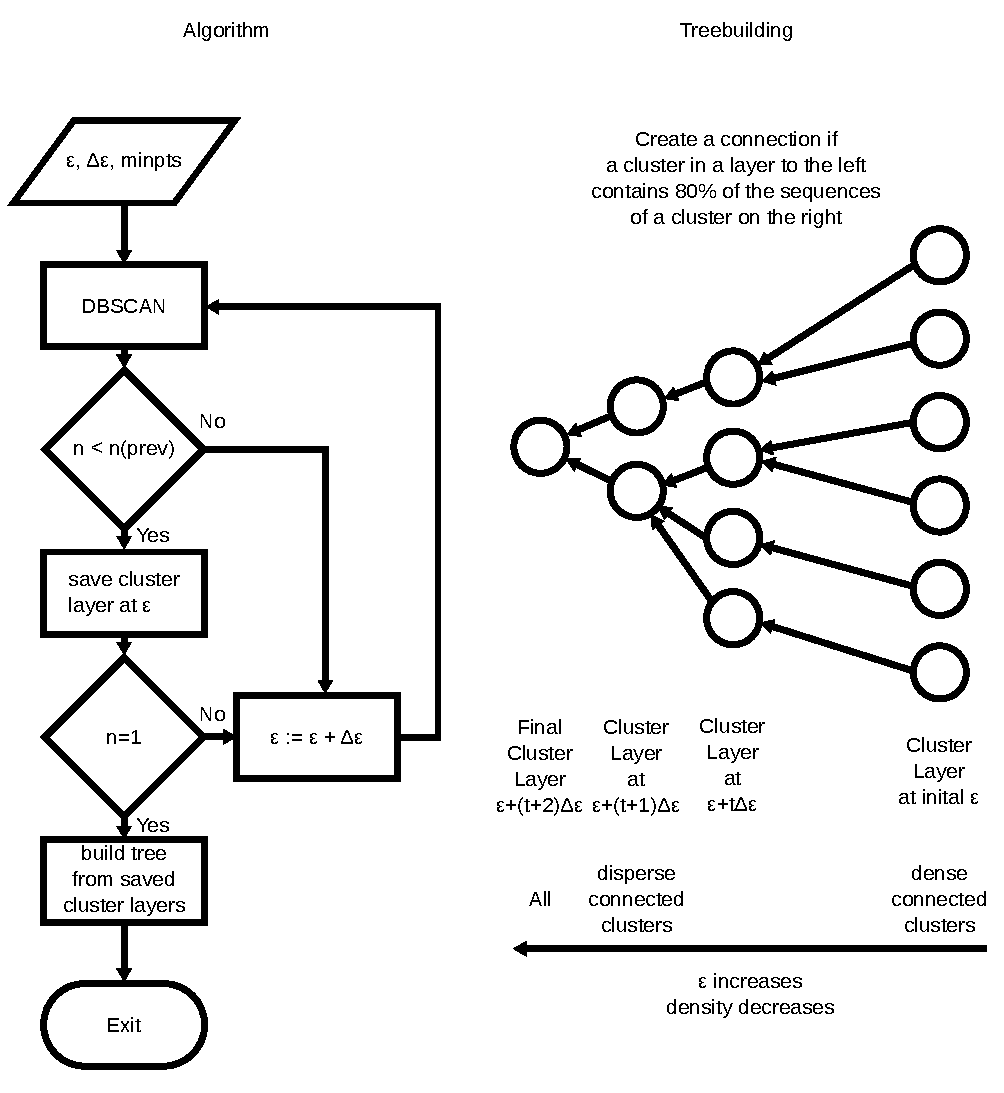
\includegraphics[scale=0.8]{algorithm.pdf}
  \end{center}
  \caption{\textbf{Building trees from sequences:} Highlights our
    algorithm, and its three parameter input $\epsilon$ the initial
    epsilon neighborhood radius for the DBSCAN algorithm, $\Delta
    \epsilon$ the increase of $\epsilon$ in every step and minpts the
    minimal number of points to be found in an epsilon neighborhood to
    either extend or create a cluster. $n$ in the
    diagram represents the number of clusters of the current DBSCAN
    run, $n(\mathrm{prev})$ the number of clusters of the previous
    run. $t$ at the treebuilding side, the stepnumber and hence, how
    often DBSCAN has been run.
    The algorithm works itself from right to the left through the
    tree, detecting first using a small $\epsilon$ very dense clusters
    of nucleic sequences and hence, clusters that are highly conserved
    in sequence. In increasing DBSCANS $\epsilon$ from layer to layer,
    the clusters contain less and less conserved sequences, and
    basically fusion from layer to layer, until DBSCAN just detects a
    single cluster, the root of the tree.}
  \label{fig-adaptive-dbscan}
\end{figure*}
The algorithm further highlights the same optimizations as pointed out
in section \ref{sec-dbscan-algorithm}. Further the algorithm is
multithreaded precalculating layers at different $\epsilon$s in
different threads in parallel.
Finally a Message Passing Interface (MPI) version of the GPU based
Smith Waterman DBSCAN region expand function exists. In this function
the distance between a sequence in question with all other sequences
of the dataset is to be evaluated to find out weather or not this
distance is smaller than $\epsilon$ and falls within an epsilon
neighborhood or not. Using the MPI interfaces the algorithm has the
possibility to profit from multiple available GPUs in multiple
machines such as in a clustering environment. We have successfully
tested to run this algorithm on six independent cluster nodes with
four GPUs each using an infiniband network backbone.

\subsection{Example}

\lstset{language=bash,
  caption={Calling the \emph{adaptive\_clustering\_PCA} tools},
  label=lst-adaptivecluster-example}
\begin{lstlisting}
adaptive_clustering_PCA test.fasta 0.02 0.01 4 /tmp/out-splits- 8 7 test.pca 
\end{lstlisting}
Performs an adaptive clustering run on the sequences stored in
test.fasta by applying DBSCAN on the 7 dimensional k-mer subspace
defined by the projections onto the principal components stored in
test.pca. The \emph{inital-epsilon} is defined to be 0.02, the
\emph{delta-epsilon} is defined to be 0.01 and a minimum number of
points for cluster expansion or creation is defined to be four.
The resulting clusters for each run are stored in binary form at
\emph{/tmp/out-splists-X} where X counts from 0 to the number of
layers calculated until only a single cluster was found due to the
small density at a large $\epsilon$.

\subsection{Implemenation}
The algorithm and its interfaces are implemented in
\emph{adaptive\_clustering.c}. The code makes heavily use of the DBSCAN
algorithm implemented in \emph{dbscan.c}. 
